\newpage
\section{Auswertung}
\label{sec:Auswertung}


\subsection{(a) Erzeugen einer amplitudenmodulierten Schwingung mit
Hilfe eines Ringmodulators}
\label{subsec:auswertung_a}
In der Abbildung \ref{fig:ringamp_zeit} ist das Modulationssignal
sowie die amplitudenmodulierte Schwingung, die mit einem Ringmodulatorschaltung \ref{fig:Ringmodulator}
erzeugt wird,
in Abhänigkeit der Zeit dargestellt.
Die Modulationsfrequenz beträgt $\SI{100(5)}{\kilo\hertz}$
und die Trägerfrequenz $\SI{1.00(5)}{\mega\hertz}$.

\begin{figure}
  \centering
  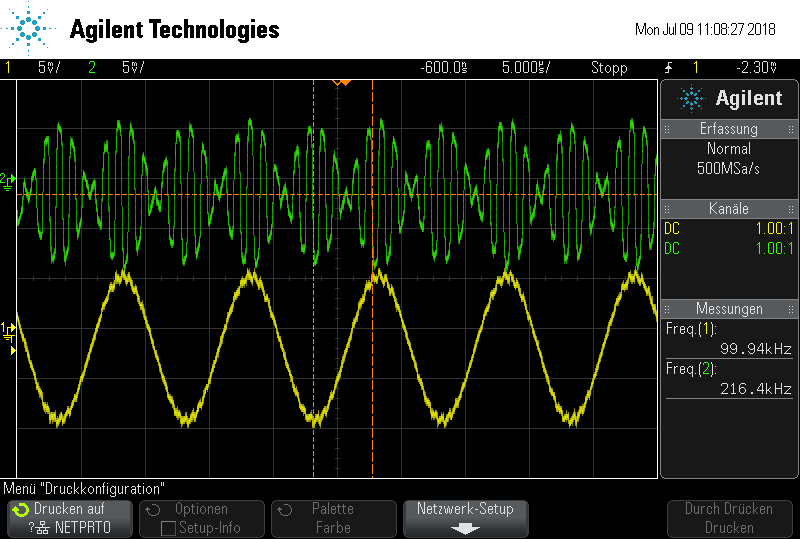
\includegraphics[width=0.7\textwidth]{osci/amp_ringmodulator.png}
  \caption{Amplitudenmodulierte
  Schwingung eines Ringmodulators und das entsprechende Modulationssignal.}
  \label{fig:ringamp_zeit}
\end{figure}

\FloatBarrier
\subsection{(b) Untersuchung des Frequenzspektrums einer
amplitudenmodulierten Schwingung}
\label{subsec:auswertung_b}

Die aus Kapitel \ref{subsec:auswertung_a} erzeugete
amplitudenmodulierte Schwingung wird in Abbildung \ref{fig:ringamp_frequenz}
im Frequenzraum dargestellt.
\begin{figure}
  \centering
  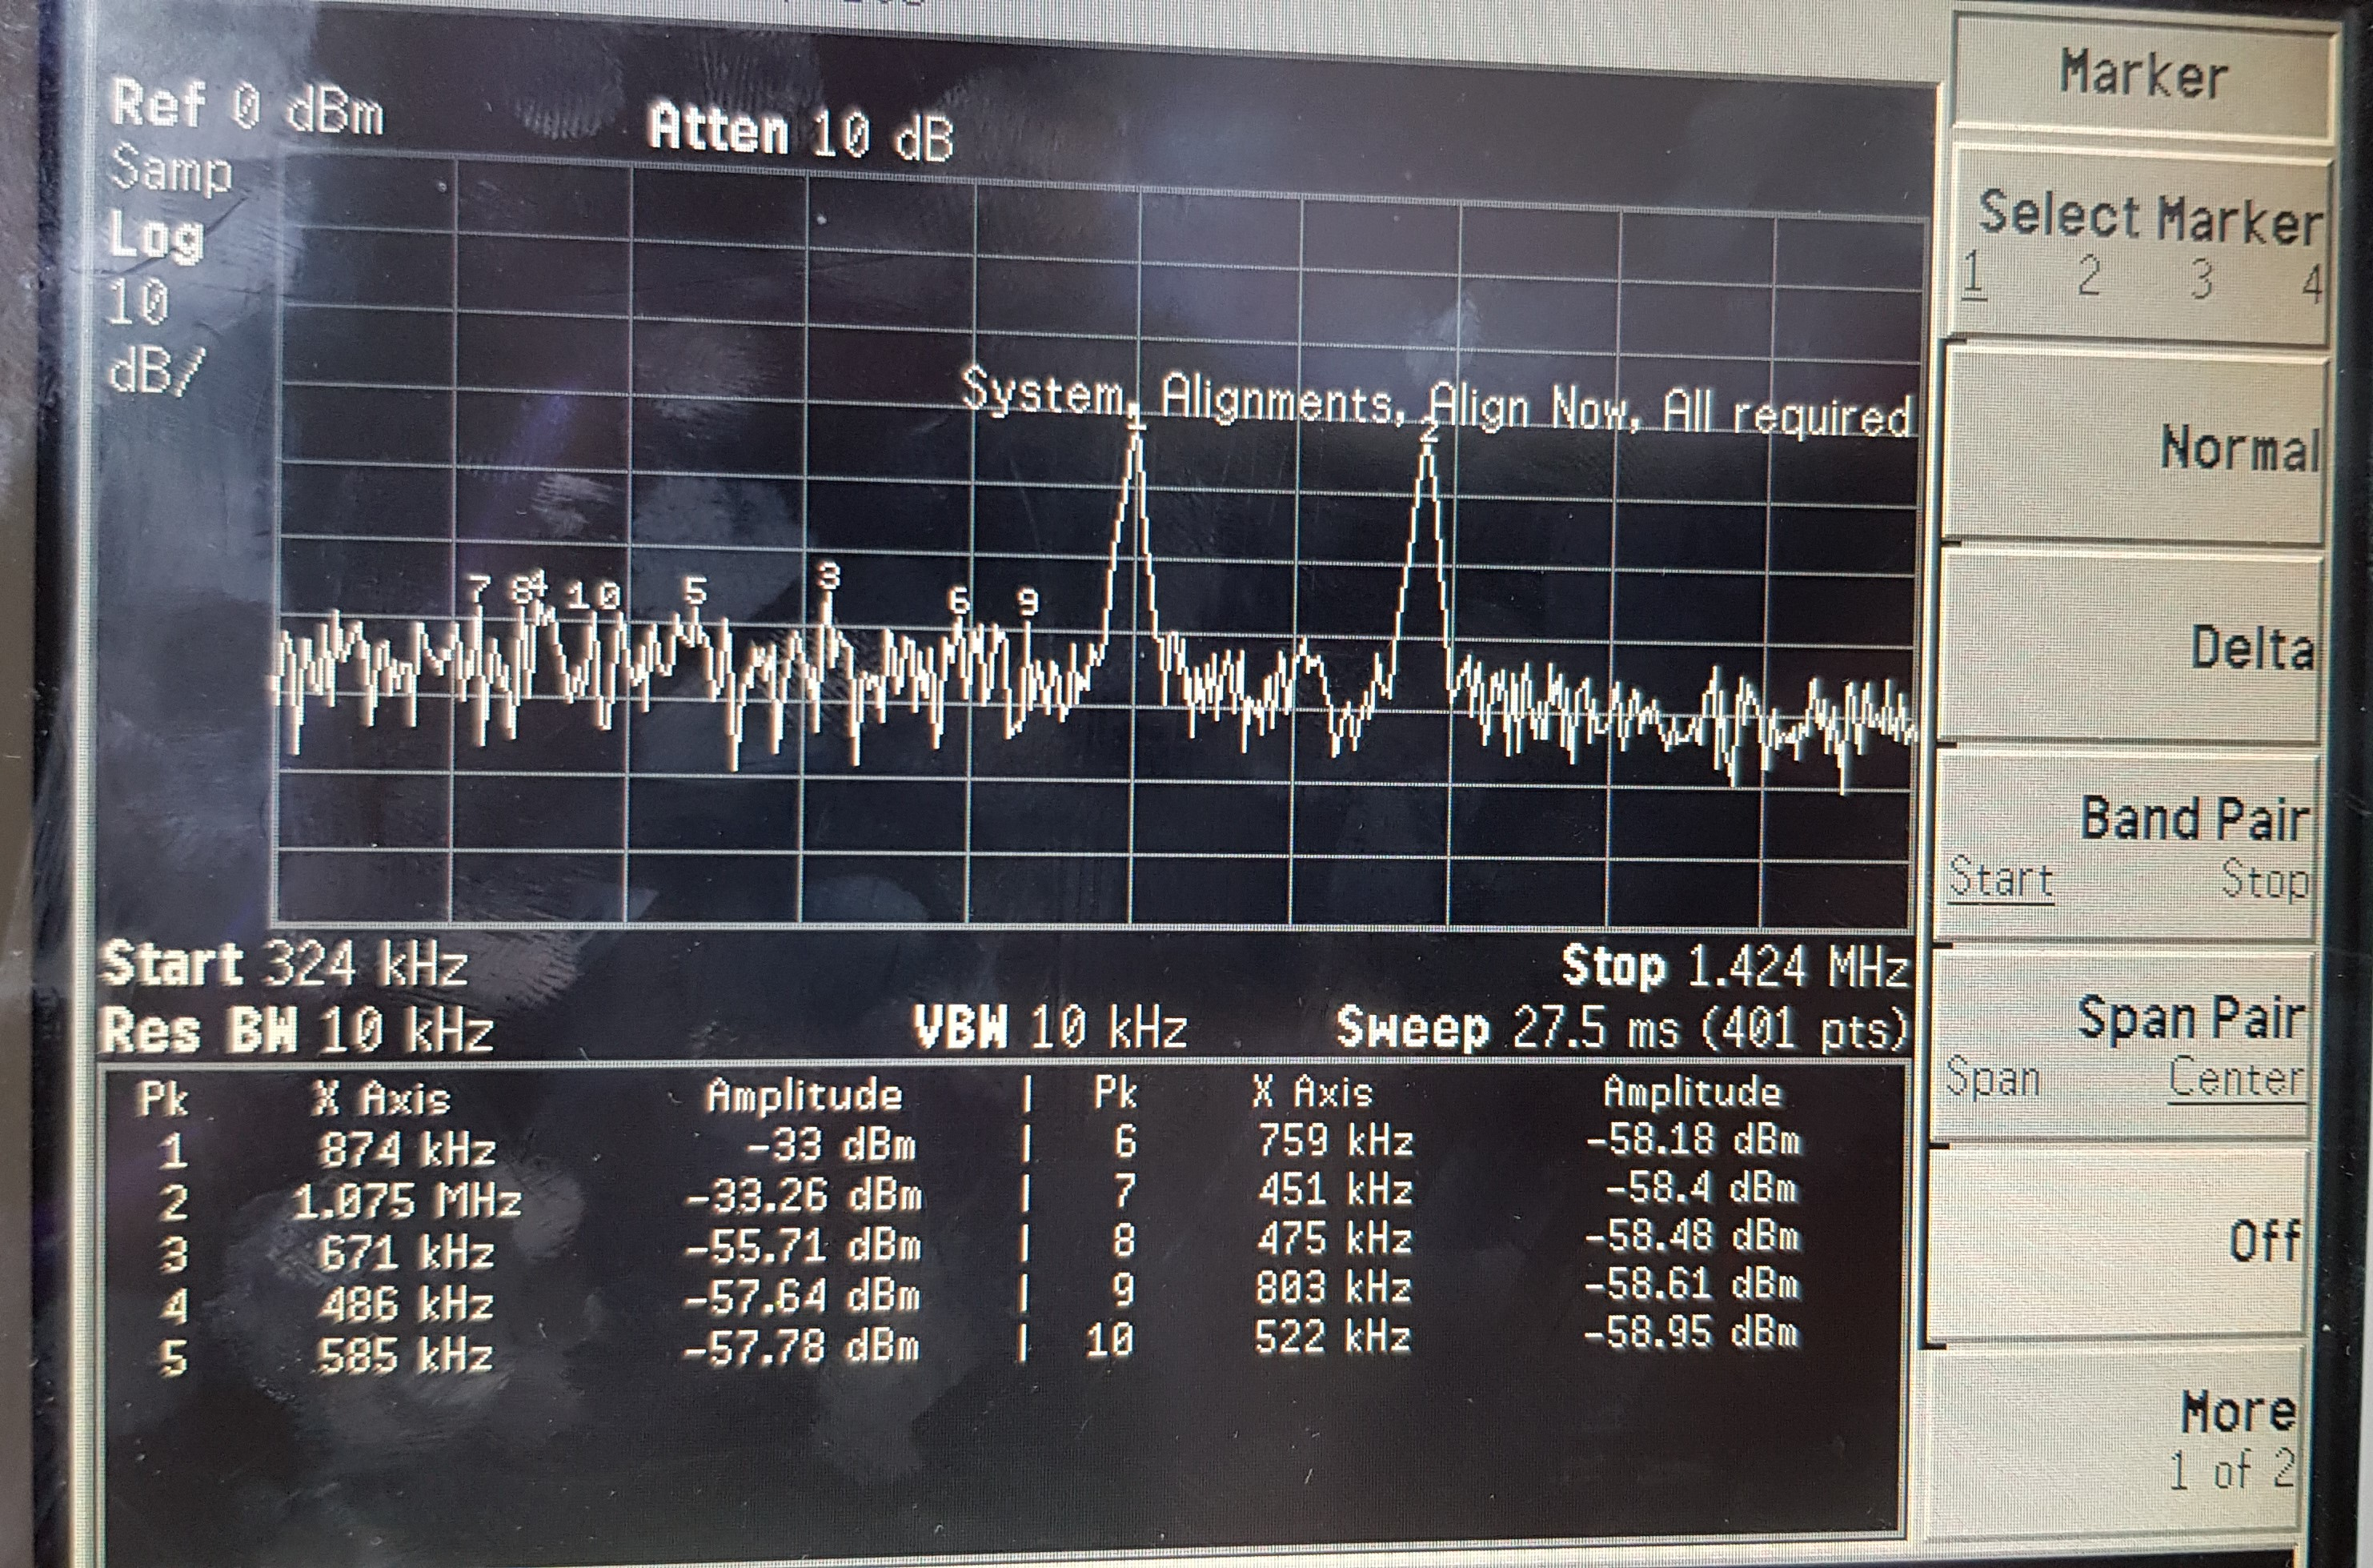
\includegraphics[width=0.7\textwidth]{spec/frequenzbereich_klein_ring.jpg}
  \caption{Amplitudenmodulierte
  Schwingung eines Ringmodulators im Frequenzraum.}
  \label{fig:ringamp_frequenz}
\end{figure}
Aus der Abbildung \ref{fig:ringamp_frequenz}
können die beiden aus der Modulation resultierenden Frequenzen
\begin{align}
  f_{\text{T}}+f_{\text{M}}&=\SI{0.87(5)}{\mega\hertz} \\
  f_{\text{T}}-f_{\text{M}}&=\SI{1.07(5)}{\mega\hertz}
\end{align}
bestimmt werden.
Deutlich wird ebendfalls das es keine Trägerabstrahlung vorliegt und
keine Terme höherer Ordnung auftreten.

\FloatBarrier
\subsection{(c) Erzeugen einer amplitudenmodulierten Schwingung
mit Hilfe einer Gleichrichterdiode}
\label{subsec:auswertung_c}
Anstelle des Ringmodulator wird eine Diode wie in Schaltung \ref{fig:14} zur Amplitudenmodulation verwendnet.
Die Abbildungen \ref{fig:diode_zeit} und \ref{fig:diode_frequenz_klein}
enthälten
sowohl das zeitabhänige Signal und das Signal im Frequenzraum.
Als Frequenzen werden $f_{\text{T}}=\SI{2.50(5)}{\mega\hertz}$ und
$f_{\text{M}}=\SI{0.10(1)}{\mega\hertz}$ mit den Amplituden
$U_{\text{T}}=\SI{1.30(5)}{\volt}$ und
$U_{\text{M}}=\SI{0.25(5)}{\volt}$.
verwendet.

\begin{figure}
  \centering
  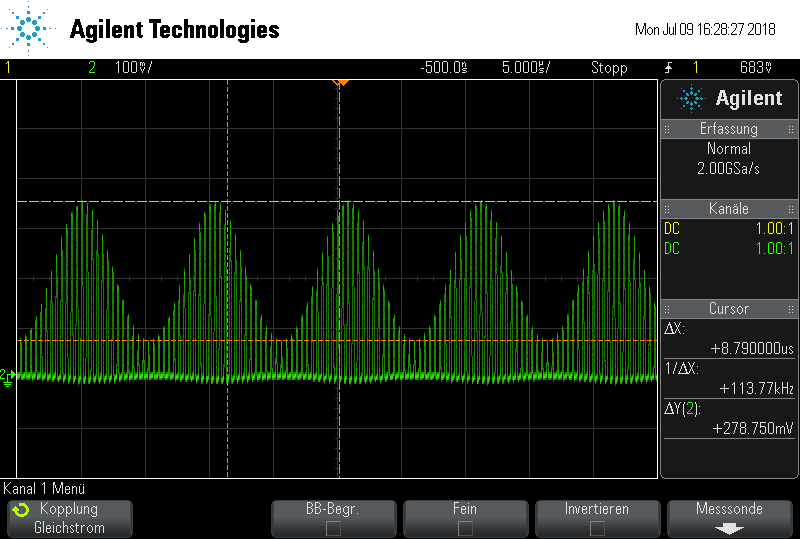
\includegraphics[width=0.7\textwidth]{osci/amp_mod_diode.png}
  \caption{Amplitudenmodulierte
  Schwingung einer Diode nach dem Aufbau aus Abb.\ref{fig:14}.}
  \label{fig:diode_zeit}
\end{figure}

Aus Abbildung \ref{fig:diode_zeit} folgt der Abstand $\Delta U$ zwischen dem maximum und minimum Einhüllenden
\begin{align}
\Delta U &= U_{\text{T}}(1+m)-U_{\text{T}}(1-m) =2U_{\text{T}}m = \SI{0.27(2)}{\volt}
\intertext{und somit für den Modulationsgrad}
    m &=  \frac{\Delta U }{2U_{\text{T}}}=  \num{0.11(1)} \label{eqn:m_oszi}
\end{align}

\begin{figure}
  \centering
  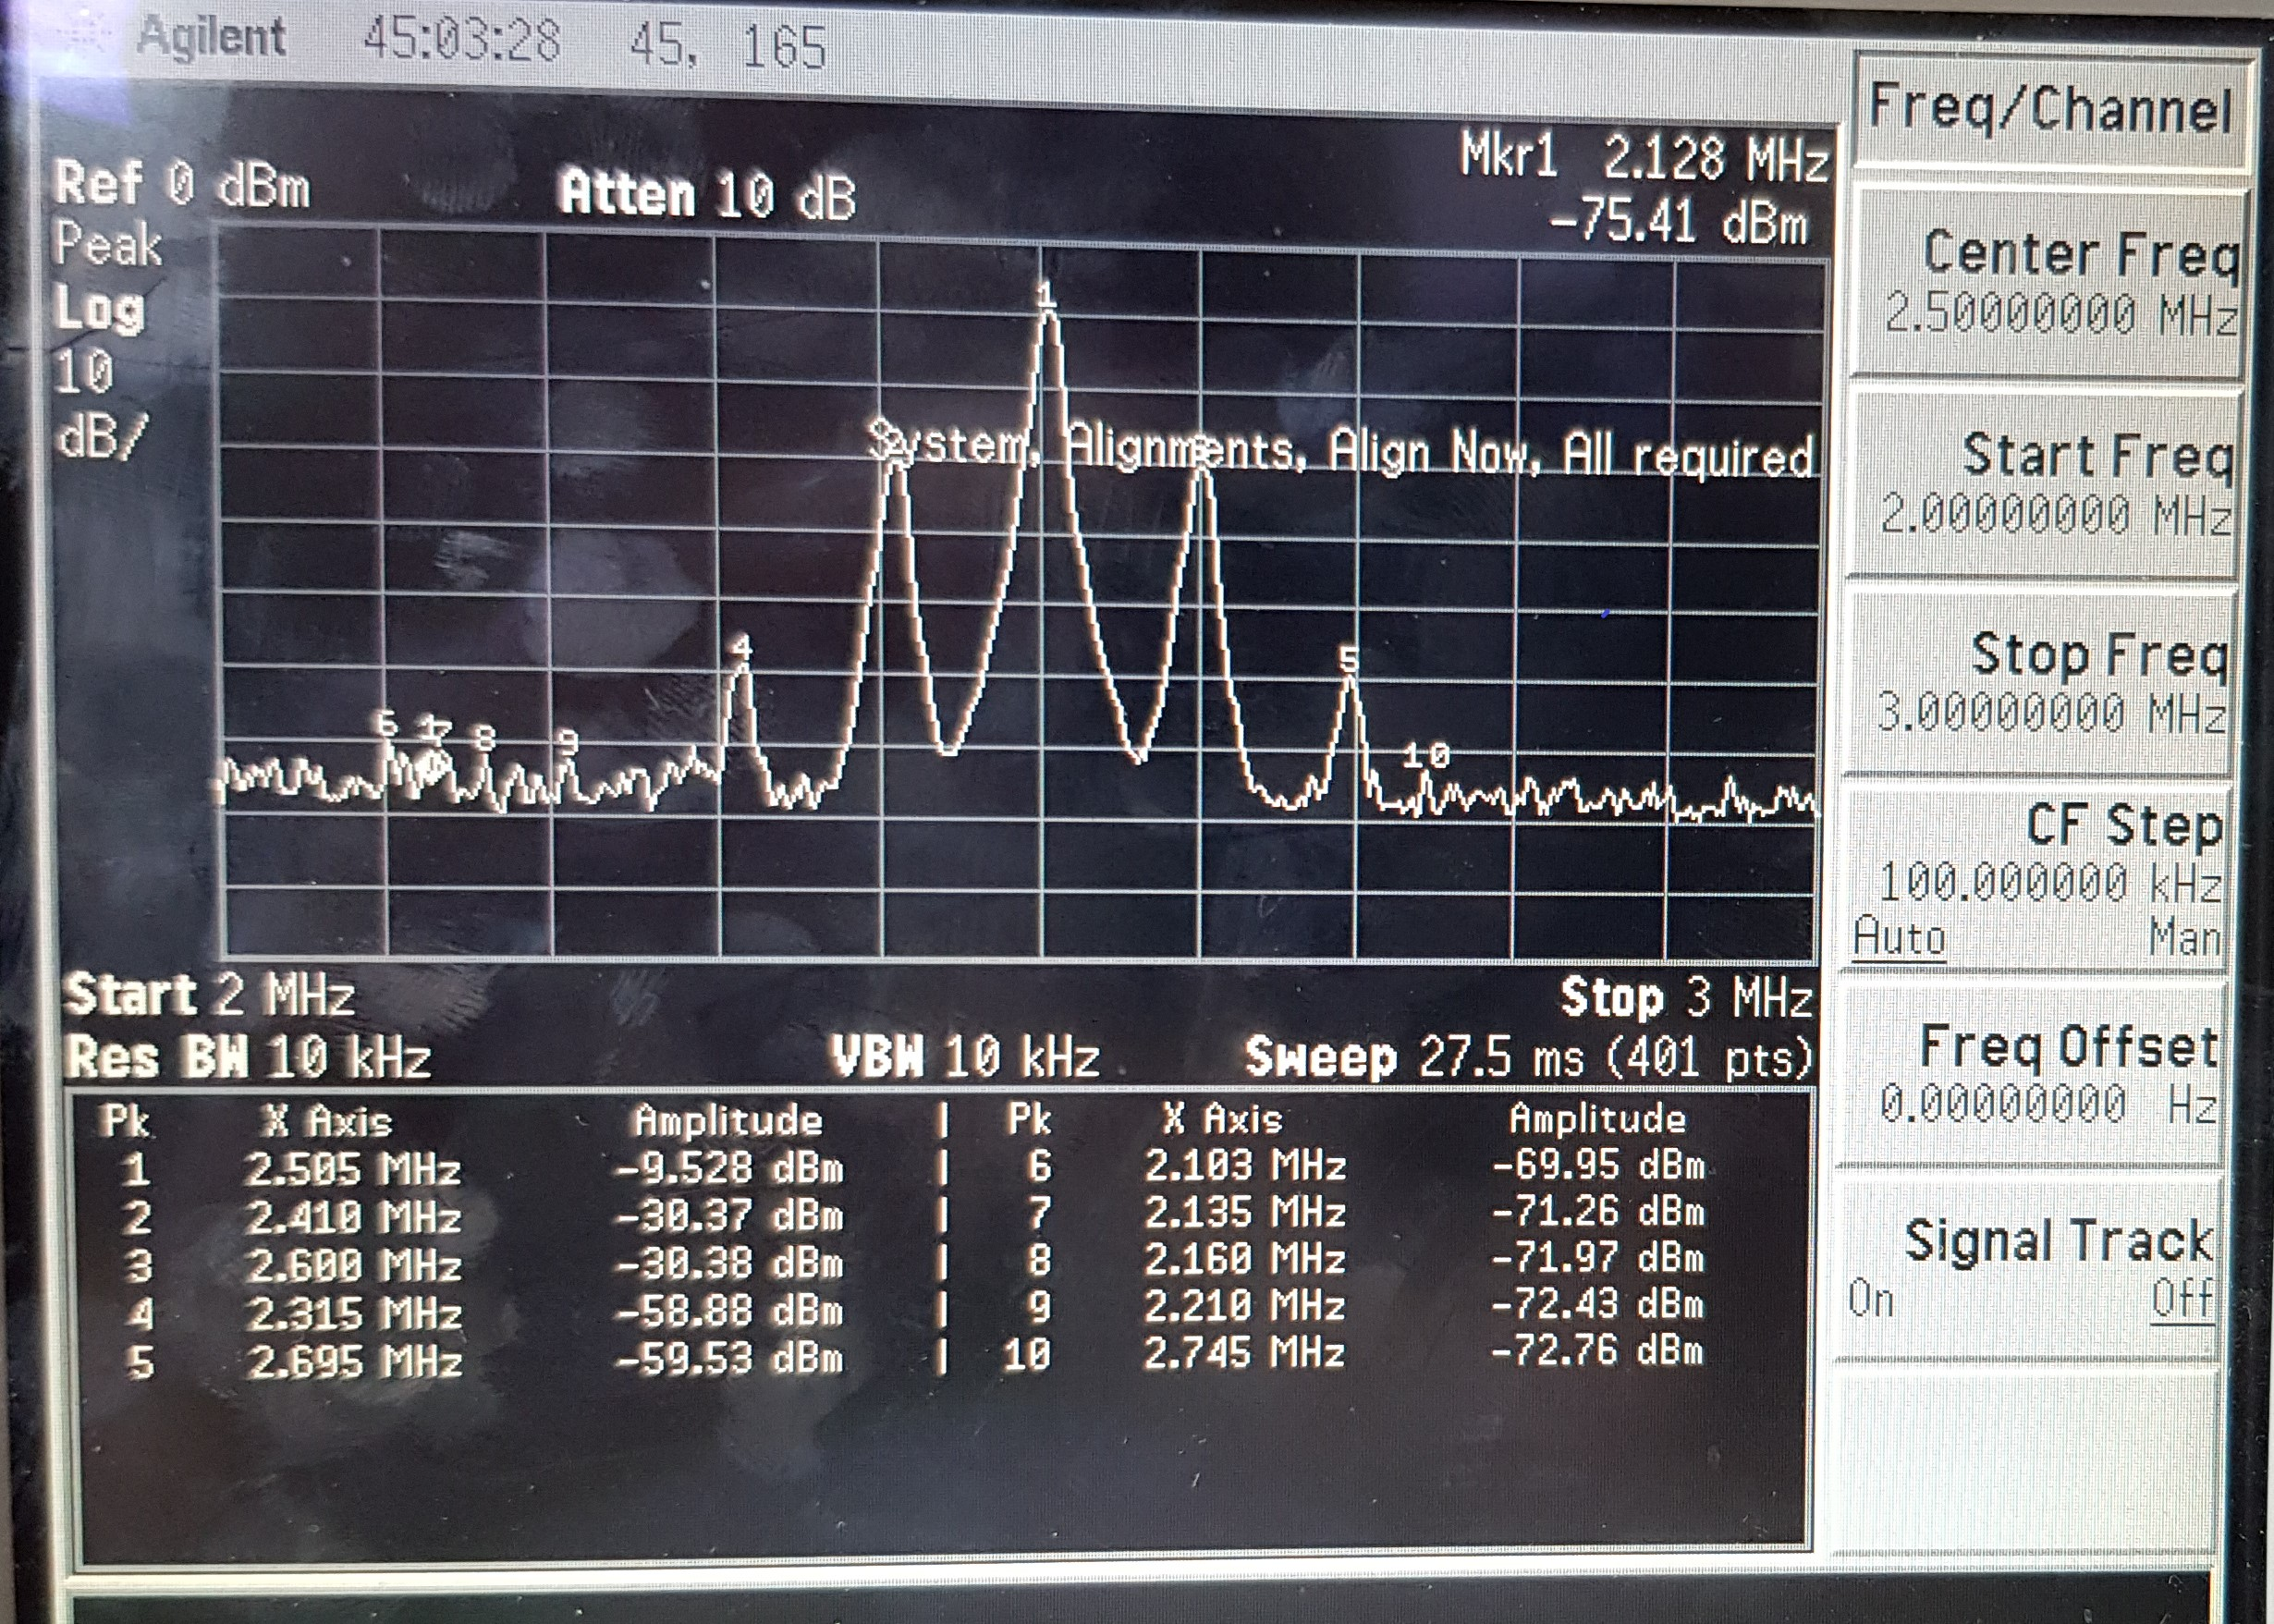
\includegraphics[width=0.7\textwidth]{spec/frequenzbereich_klein_diode.jpg}
  \caption{Amplitudenmodulierte
Schwingung einer Diode im Frequenzraum.}
  \label{fig:diode_frequenz_klein}
\end{figure}
Aus der Abbildung \ref{fig:diode_frequenz_klein}
wird die Trägerabstrahlung
sowie
die auftetenden Mischterme durch die nicht linerare
Kennlinie
der Diode deutlich.
Die Abbildung \ref{fig:diode_frequenz_gross}
für einene größeren Frequenzbereich
verdeutlich dies ebenfalls, da Terme bis
zu $\mathcal{O}\left(U^4\right)$
also Frequenzen mit beispielsweise $4f_{\text{T}}$
deutlich sichtbar sind.
\begin{figure}
  \centering
  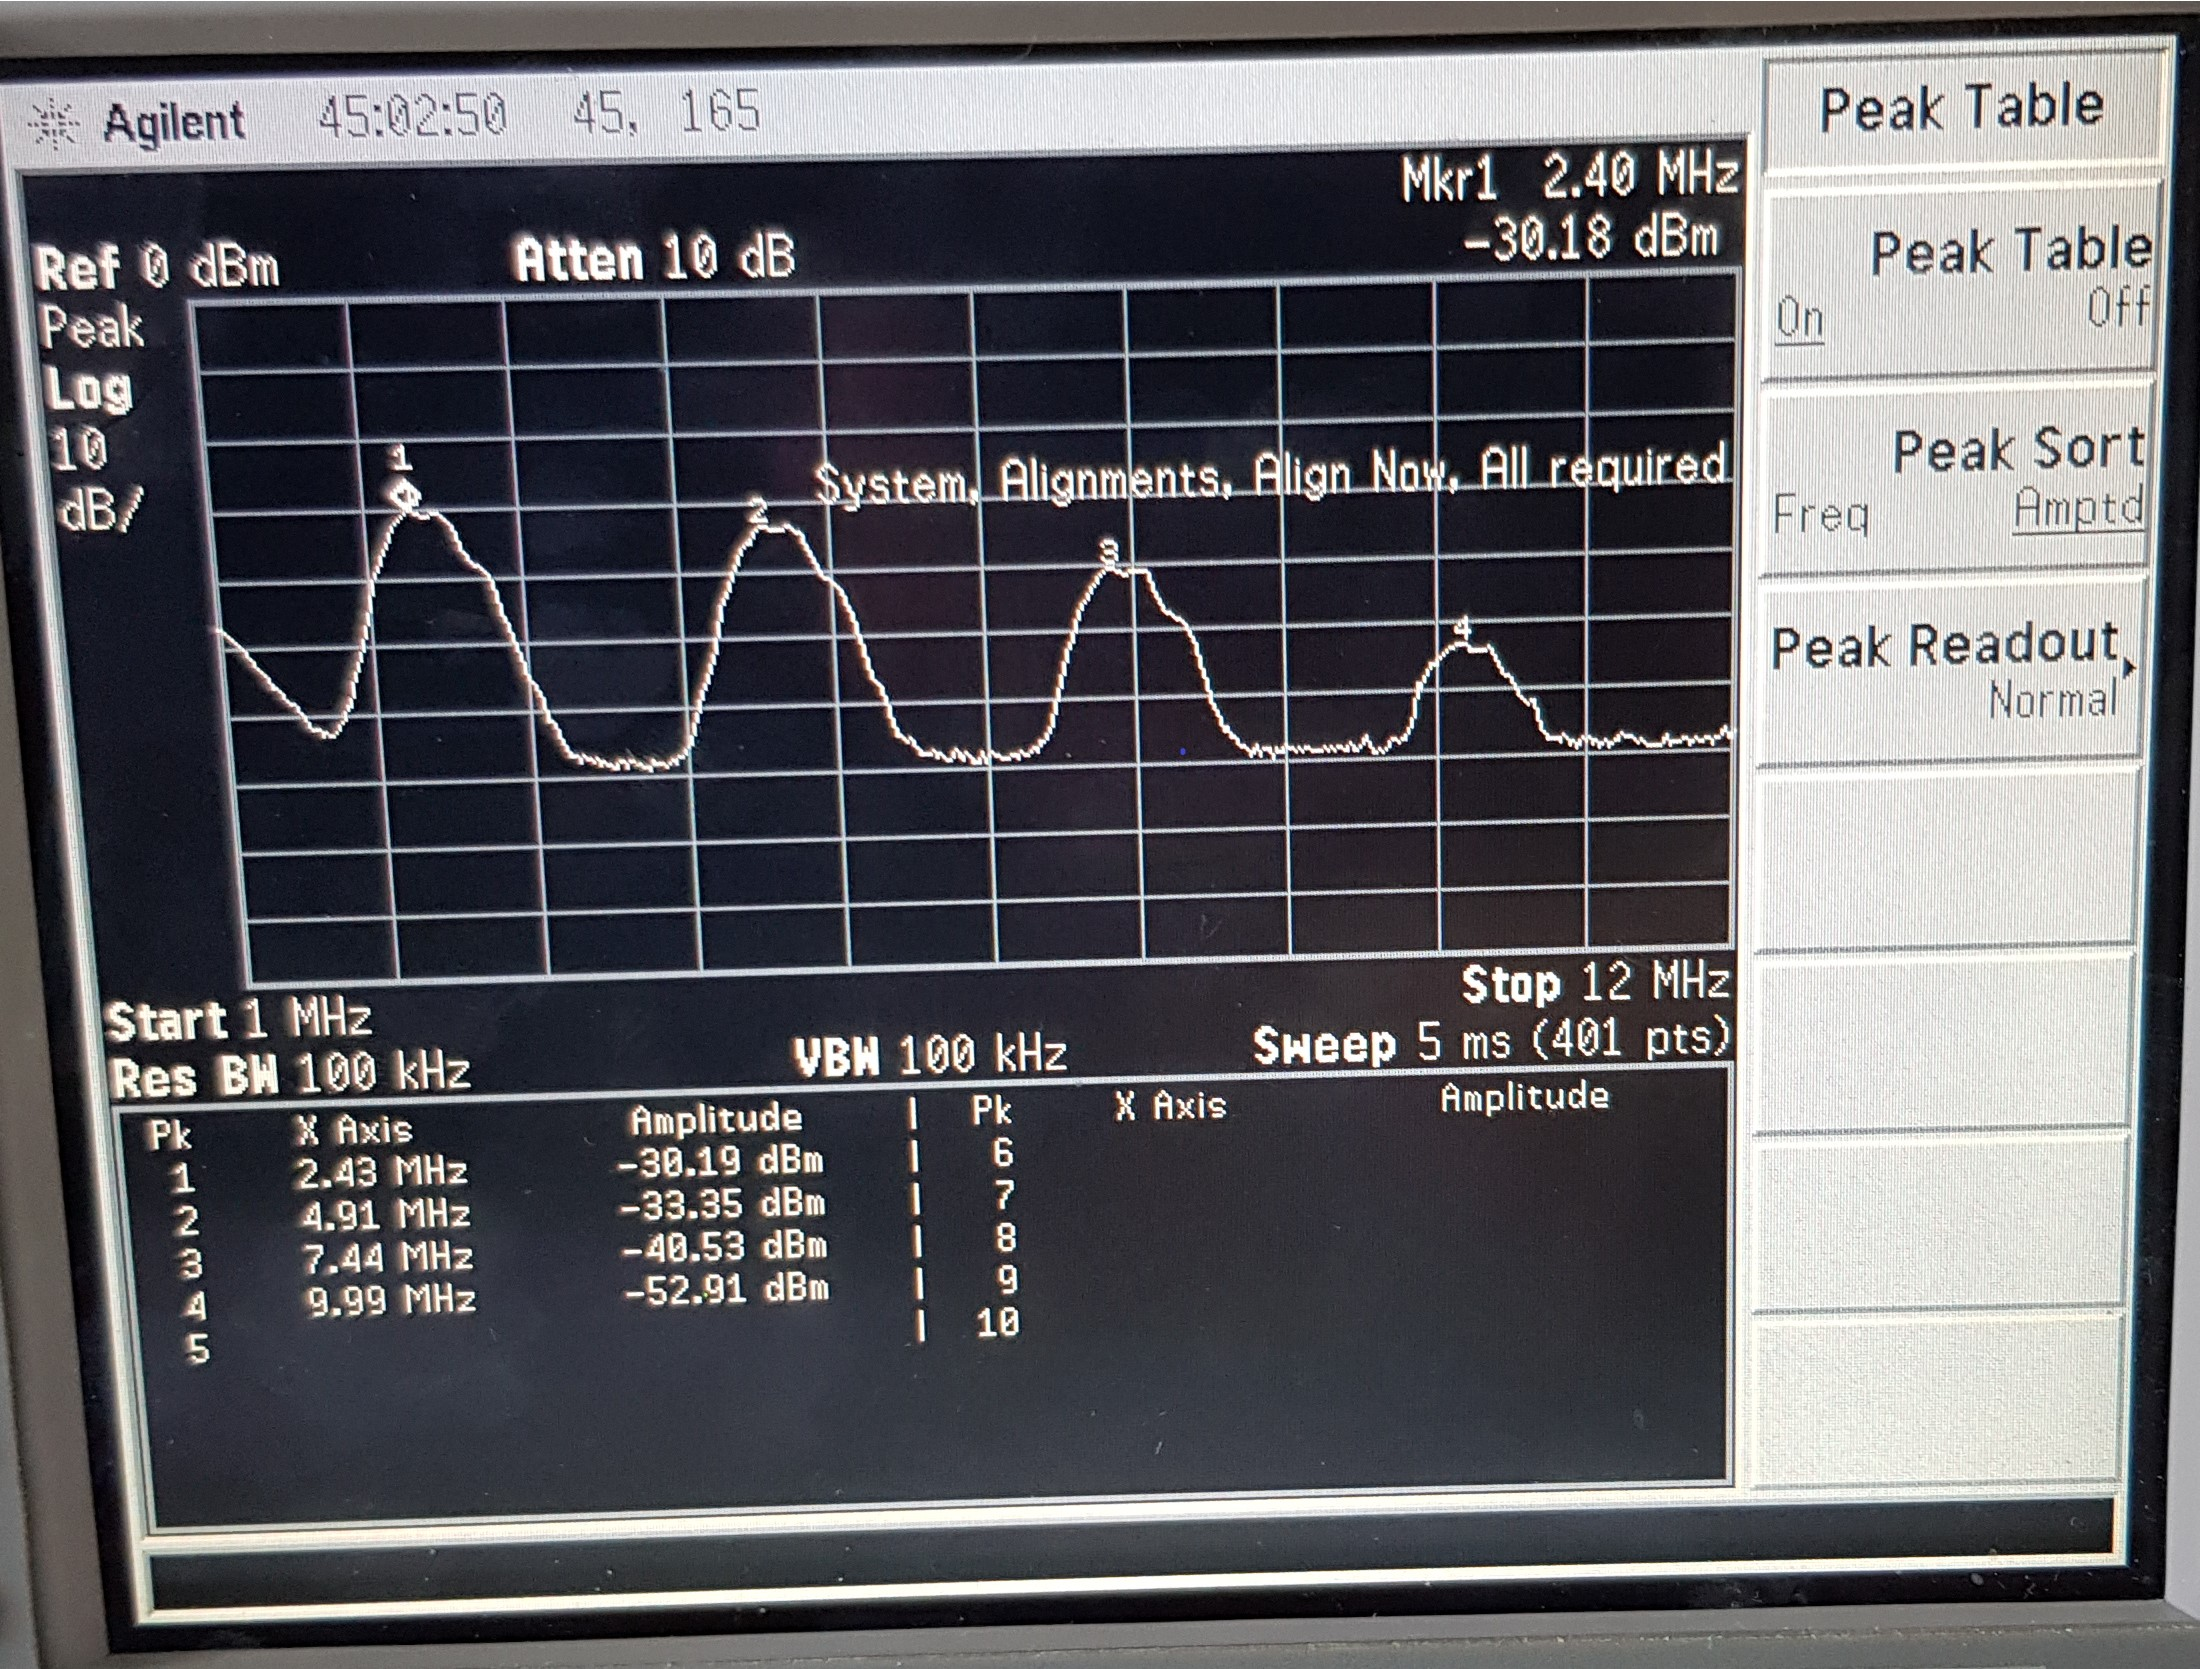
\includegraphics[width=0.7\textwidth]{spec/frequenzbereich_gross_diode.jpg}
  \caption{Amplitudenmodulierte
Schwingung einer Diode im Frequenzraum mit Oberschwingungen.}
\label{fig:diode_frequenz_gross}
\end{figure}

Ebenfalls wird der Modulationsgrad $m$ aus den Frequenzspektrum bestimmt.
Für die Spannung der Peaks bei den Frequenzen $\omega_{\text{T}}-\omega_{\text{M}}$ ,$\omega_{\text{T}}$  und $\omega_{\text{T}}+\omega_{\text{M}}$
gilt der in Abbildung \ref{fig:2} dargestellte
Zusammenhang.

\begin{figure}
  \centering
  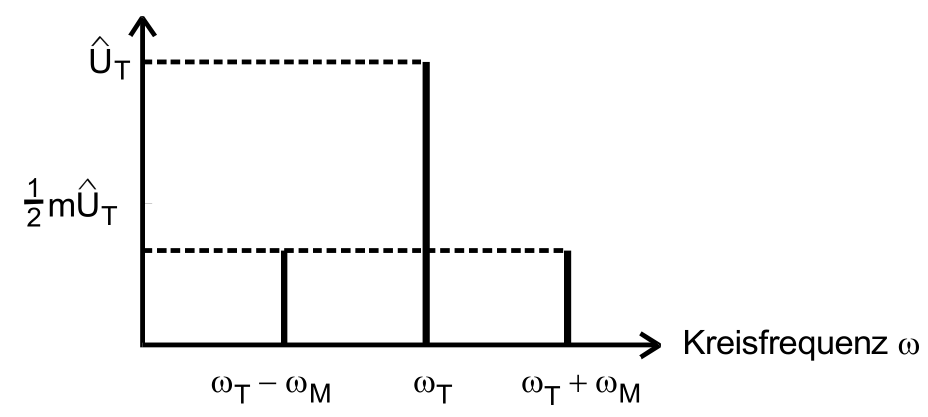
\includegraphics[width=0.7\textwidth]{figures/frequenzspektrum.PNG}
  \caption{Frequenzspektrum für eine amplitudenmoduliertes Signal.}
  \label{fig:2}
\end{figure}

Aus der Abbildung \ref{fig:diode_frequenz_klein} können die Leistungen
\begin{align}
  % \si{\deci\belmilliwatt}
  % \si{\dBm}
P_{f_{\text{T}}-f_{\text{M}}}&=\SI{-9.53(5)}{\deci\belmilliwatt}\\
P_{f_{\text{T}}}&=\SI{-30.37(5)}{\deci\belmilliwatt}\\
P_{f_{\text{T}}+f_{\text{M}}}&=\SI{-30.38(5)}{\deci\belmilliwatt}
\end{align}
der entsprechenden Frequenzen entnommen werden.
Für die Spannungen ergibt sich dann nach
\begin{align}
  U= \sqrt{P R}
\end{align}
die folgenden Werte
\begin{align}
   \hat{U}_{f_{\text{T}}-f_{\text{M}}}&=\sqrt{R}\SI{0.957(6)}{\milli\volt\per\sqrt{\ohm}}\\
  \hat{U}_{f_{\text{T}}}&=\sqrt{R}\SI{10.56(6)}{\milli\volt\per\sqrt{\ohm}}\\
  \hat{U}_{f_{\text{T}}+f_{\text{M}}}&=\sqrt{R}\SI{0.958(6)}{\milli\volt\per\sqrt{\ohm}}.
\end{align}
Die beiden äußeren Spannungen werden gemittelt
\begin{align}
  \overline{\hat{U}_{f_{\text{T}}\pm f_{\text{M}}}} = \sqrt{R}\SI{0.9577(4)}{\milli\volt\per\sqrt{\ohm}}
\end{align}
und für
dem Modulationsgrad $m$ ergibt sich
\begin{align}
m=\frac{2\overline{\hat{U}_{f_{\text{T}}\pm f_{\text{M}}}}}{U_{f_{\text{T}}}} = \num{0.182(1)}. \label{eqn:m_leistung}
\end{align}
Aus den beiden bestimmten Modulationsgraden aus \eqref{eqn:m_oszi} und \eqref{eqn:m_leistung}ergibt sich der Mittelwert
\begin{align}
\overline{m}=\num{0.143(2)}.
\end{align}

\FloatBarrier
\subsection{(d) Erzeugen einer frequenzmodulierten Schwingung}
\label{subsec:auswertung_d}
Die Abbildung \ref{fig:freq_zeit} enthält eine zeitabhänige frequenzmodulierte
Schwingung, die durch die Schaltung aus Abbildung \ref{fig:6}
gebildet wird.
Da für die  $\SI{90}{\degree}$-Phasenverschiebung ein Laufzeitkabel mit der
Zeit T=$\SI{250}{\nano\second}$ verwendet wird, muss somit die
Trägerfrequenz gerade genau $f_{\text{T}} = \SI{1.00(5)}{\mega\hertz}$
betragen, um eine Phasenverschiebung um $\SI{90}{\degree}$
zu erzeugen. Als Modulationsfrequenz wird
$f_{\text{M}}=\SI{0.10(1)}{\mega\hertz}$ verwendet.

\begin{figure}
  \centering
  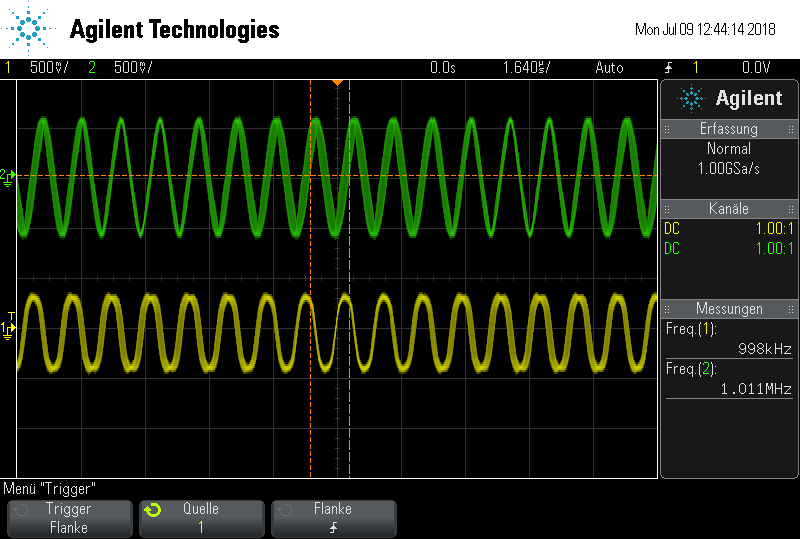
\includegraphics[width=0.7\textwidth]{osci/freq_mod.png}
  \caption{Trägerspammung ($U_{\text{T}}$ gelb) und Frequenzmodulierte
  Schwingung($U_3$ grün), die nach dem Aufbau aus Abb.\ref{fig:Ringmodulator_frequenz} erzeugt wird.}
  \label{fig:freq_zeit}
\end{figure}
Der Modulationsgrad $m$ wird
bei der Frequenzmodulation
aus der maximalen Verschmierung
$\Delta t=t_2-t_1$ in x-Richtung des Signals bestimmt
und der Modulationsfrequenz $f_{\text{M}}$.
Die sichtbare Verschmierung in der
Abbildung \ref{fig:freq_zeit}
entsteht durch die unterschiedlichen
Funktionsscharen von $U(t)_{\phi}$ die
die zeitabhänige Kreisfrequenz
\begin{align}
\omega(t)_{\phi}=\omega_\text{T}\left(1-m\sin(\omega_\text{M}t + \phi)\right)\\
\end{align}
beitzten aber mit unterschiedlichen Phasen $\phi$ starten.
Dies hat zu Folge das die Funktionen zu Beginn
auseinanderlaufen, somit die Verschmierung
zunimmt, um danach wieder
zusammenzulaufen.
Die Verschmierung liegt zwischen
der Schwingung mit den Frequenzen
$\omega_{\phi=\pi}(t)$
und $\omega_{\phi=0}(t)$.
Die Verschmierung
wird für die
Werte $t_1=\frac{\pi}{ \omega_{\text{M}}}$
und $t_2 = t_1+\Delta t$ maximal.
Die Gesamtphase $\Phi$ der Schwingung $U(t)$
zu Zeitpunkt $t$
ergibt sich aus
\begin{align}
  \Phi(t)&= \int_0^t \omega(t).
\intertext{Da die Verschmierung
horizontal gemessen wird
befindet sich die Schwingungen in der gleichen
Gesamtphase}
\Phi(t_1)_{\phi=\pi}&=\Phi(t_2)_{\phi=0}\\
\int_0^{t_1} \omega(t)_{\phi=\pi} \symup{d}t &= \int_0^{t_2} \omega(t)_{\phi=0} \symup{d}t.
\intertext{durch Einsetzten von $t_1$ und $t_2$ für die maximale Verschmierung folgt für
den Modulationsgrad}
m = \frac{\Delta t \omega_{\text{M} }}{3+\cos\omega_{\text{M}}\Delta t}
&=\frac{2\pi\Delta t f_{\text{M} }}{3+\cos2\pi f_{\text{M}} \Delta t}. \label{eqn:modu_freq}
\intertext{Aus der Abbildung \ref{fig:freq_zeit} wird die maximale Verschmierung
zu}
\Delta t &= \SI{250(5)}{\nano\second}
\intertext{bestimmt.
Für den Modulationsgrad $m$ folgt aus Gleichung \eqref{eqn:modu_freq}}
m &= \num{0.039(4)}.
\end{align}

Die Abbildung \ref{fig:frequenz_freq} enthält die frequenzmodulierte Schwingung
im Frequenzraum.
\begin{figure}
  \centering
  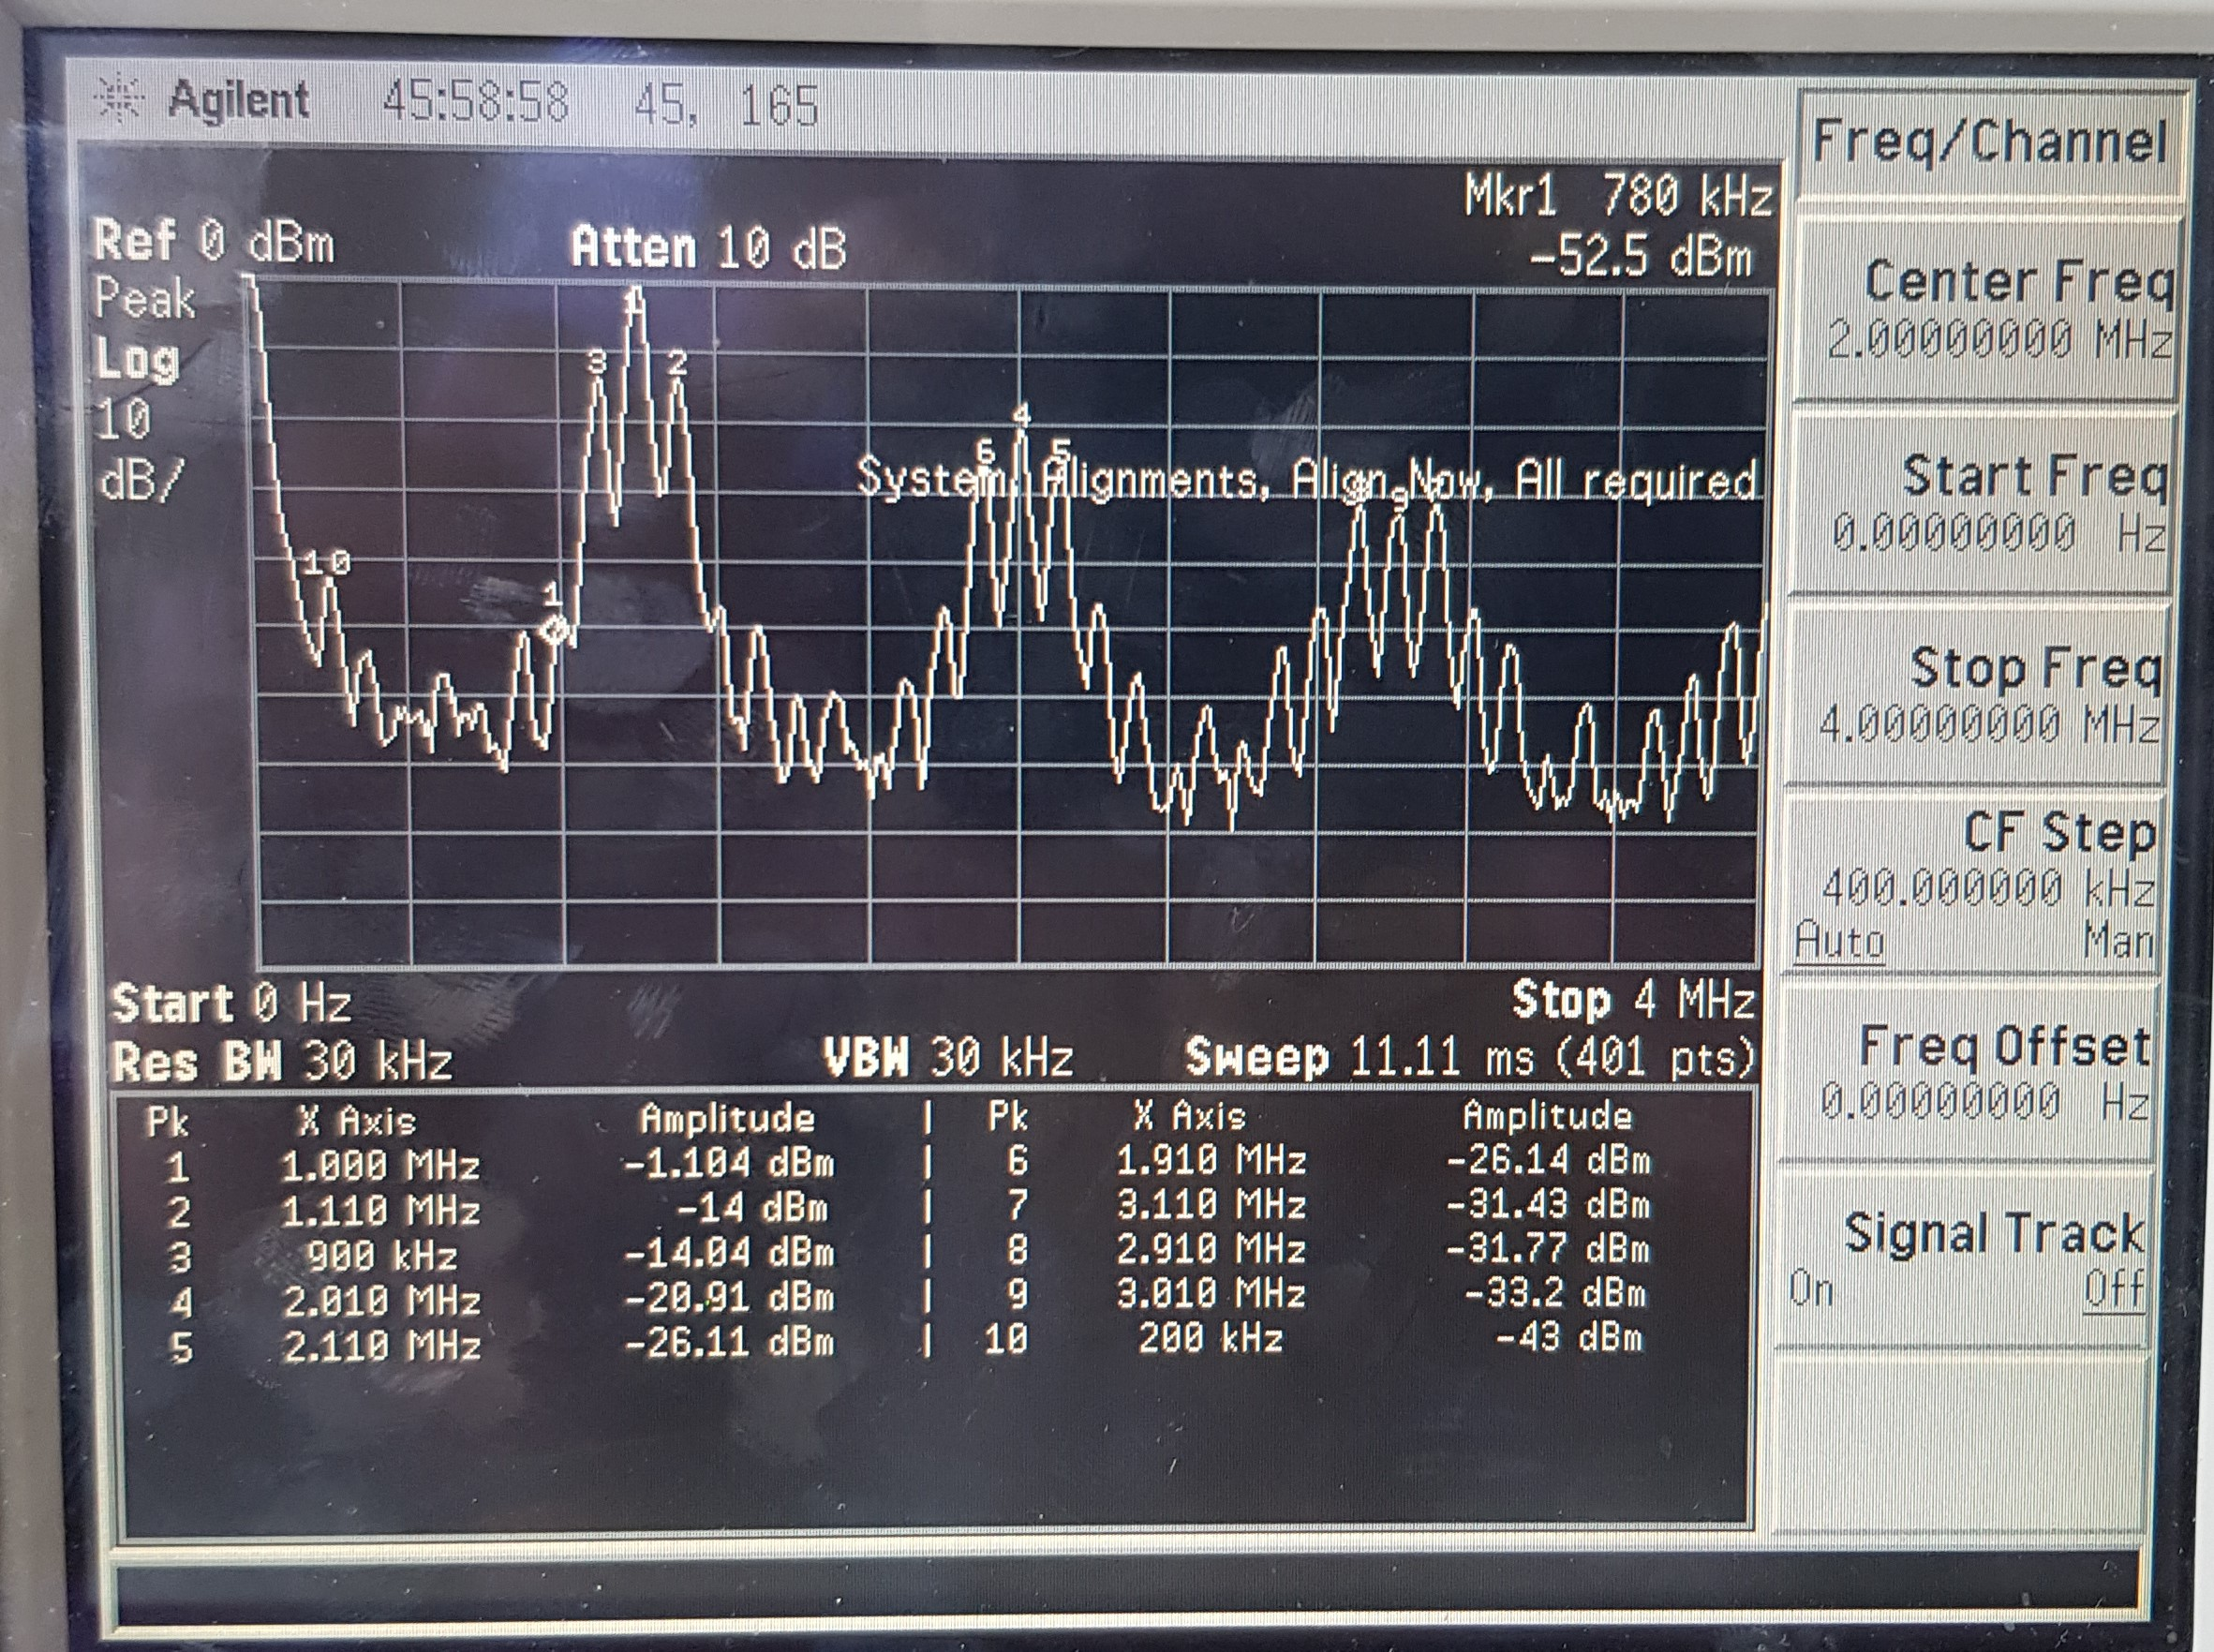
\includegraphics[width=0.7\textwidth]{spec/frequenzmodulation_bereich_fresh_cool.jpg}
  \caption{Frequenzmodulierte
Schwingung im Frequenzraum.}
\label{fig:frequenz_freq}
\end{figure}
Ebenfalls sind die Mischterme sowie die Trägerabstrahlung erkennbar.
Deweiteren kann der Modulationsgrad wieder
über die Leistungsamplituden berechnet werden.
Für ein Frequenzmoduliertes Signal gilt jedoch der Zusammmenhang
\begin{align}
m=\frac{2\overline{\hat{U}_{f_{\text{T}}\pm f_{\text{M}}}}}{U_{f_{\text{T}}}} \frac{f_{\text{M}}}{f_{\text{T}}}. \label{eqn:m_leistung_f}
\end{align}
Für die Amplituden der entsprechenden Frequenzen
folgt aus Abbildung \ref{fig:frequenz_freq}
\begin{align}
  % \si{\deci\belmilliwatt}
  % \si{\dBm}
P_{f_{\text{T}}-f_{\text{M}}}&=\SI{-1.10(5)}{\deci\belmilliwatt}\\
P_{f_{\text{T}}}&=\SI{-14.00(5)}{\deci\belmilliwatt}\\
P_{f_{\text{T}}+f_{\text{M}}}&=\SI{-14.04(5)}{\deci\belmilliwatt}.
\end{align}
Die Spannungen sind somit
\begin{align}
   \hat{U}_{f_{\text{T}}-f_{\text{M}}}&=\sqrt{R}\SI{0.0316(1)}{\milli\volt\per\sqrt{\ohm}}\\
  \hat{U}_{f_{\text{T}}}&=\sqrt{R}\SI{0.031(1)}{\milli\volt\per\sqrt{\ohm}}\\
  \hat{U}_{f_{\text{T}}+f_{\text{M}}}&=\sqrt{R}\SI{0.031(1)}{\milli\volt\per\sqrt{\ohm}}
\end{align}
und der Mittelwert der äußeren Spannungen ist
\begin{align}
  \overline{\hat{U}_{f_{\text{T}}\pm f_{\text{M}}}} = \sqrt{R}\SI{0.031(0)}{\milli\volt\per\sqrt{\ohm}}.
\end{align}
Für
dem Modulationsgrad $m$ ergibt sich
\begin{align}
m=\num{0.20(1)}.
\end{align}
Aus den beiden bestimmten Modulationsgraden
ergibt sich der Mittelwert
\begin{align}
\overline{m}=\num{0.12(6)}.
\end{align}




\FloatBarrier
\subsection{(e) Untersuchung der Phasenabhängigkeit eines
phasenempfindlichen Gleichrichters}
\label{subsec:auswertung_e}
Durch die Schaltung \ref{fig:schaltung_e} wird ein phasenempfindlicher
Gleichrichter erzeugt. Um die Phase \phi zwischen
$\SI{0}{\degree}$ bis $\SI{360}{\degree}$ zu varieren, wird
auf Grund des Laufzeitkabel mit festem T=$\SI{250}{\nano\second}$
die Frequenz im Bereich von $\SI{1}{\mega\hertz}$-$\SI{5}{\mega\hertz}$
durchlaufen. Die Tablle \ref{tab:messwerte} enthält die gemessenen
Gleichspannungen $U_{\text{G}}$ für die entsprechende Phase $\phi$ und Frequenz $f$.
In der Abbildung \ref{fig:plot} ist die Gleichspannungen $U_{\text{G}}$
gegen die Phase aufgetragen.
\begin{table}
  \centering
  \caption{Messwerte der Gleichspannungen $U_{\text{G}}$, Phase \phi und Frequenz.}
  \label{tab:messwerte}
\begin{tabular}{c c c|}
\toprule
$f/\si{\mega\hertz}$ & $\phi / \si{\degree}$ &$ U_{\text{G}}/ \si{\milli\volt}$ \\
  \midrule
   1.0	&	90.0	&	13.0   \\
   1.2	&	108.0	&	34.7   \\
   1.4	&	126.0	&	50.7   \\
   1.6	&	144.0	&	60.0   \\
   1.8	&	162.0	&	67.0   \\
   2.0	&	180.0	&	69.1   \\
   2.2	&	198.0	&	61.7   \\
\bottomrule
\end{tabular}
\begin{tabular}{|c c c|}
  \toprule
  $f/\si{\mega\hertz}$ & $\phi / \si{\degree}$ &$ U_{\text{G}}/ \si{\milli\volt}$ \\
    \midrule
   2.4	&	216.0	&	45.3   \\
   2.6	&	234.0	&	21.2   \\
   2.8	&	252.0	&	2.1   \\
   3.0	&	270.0	&	-18.8   \\
   3.2	&	288.0	&	-36.5   \\
   3.4	&	306.0	&	-50.9   \\
   3.6	&	324.0	&	-60.3   \\
   \bottomrule
   \end{tabular}
  \begin{tabular}{|c c c}
    \toprule
    $f/\si{\mega\hertz}$ & $\phi / \si{\degree}$& $ U_{\text{G}}/ \si{\milli\volt}$ \\
      \midrule
   3.8	&	342.0	&	-64.4   \\
   4.0	&	0.0	&	-65.5   \\
   4.2	&	18.0	&	-58.0   \\
   4.4	&	36.0	&	-43.2   \\
   4.6	&	54.0	&	-21.0   \\
   4.8	&	72.0	&	0.5   \\
   5.0	&	90.0	&	21.9   \\
\bottomrule
\end{tabular}
\end{table}


\begin{figure}
  \centering
  \includegraphics[width=0.7\textwidth]{build/plot.pdf}
  \caption{Gemessener Gleichstrom $U_{\text{G}}$ in Abhängigkeit von der Phase.}
  \label{fig:plot}
\end{figure}


\FloatBarrier
\subsection{(f) Demodulation einer amplitudenmodulierten Schwingung
mit Hilfe eines Ringmodulators}
\label{subsubsec:auswertung_f}
Die Demudaltion mit einem Ringmodulators wird mit der Schaltung
aus Abbildung \ref{fig:demodulatorschaltung} durchgeführt. Das Ergebniss ist
in der Abbildung \ref{fig:amp_demod_ring} dargestellt.
Dabei beträt die Trägerfrequenz $f_{\text{T}}=\SI{1.00(5)}{\mega\hertz}$
und Modulationsfrequenz $f_{\text{M}}=\SI{0.10(1)}{\mega\hertz}$.


\begin{figure}
  \centering
  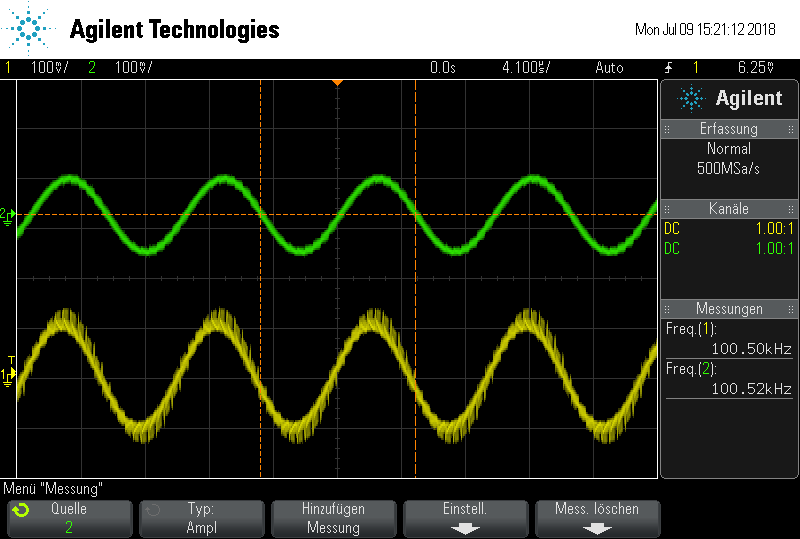
\includegraphics[width=0.7\textwidth]{osci/amp_demod.png}
  \caption{Demodulation von einem amplitudenmoduliertem Signal mit Hilfe eines
  Ringmodulator nach Schaltung \ref{fig:demodulatorschaltung}. Dargestellt ist das demodulierte Signal(grün) so wie das zu modulierende Signal.}
  \label{fig:amp_demod_ring}
\end{figure}




\FloatBarrier
\subsubsection{(g) Demodulation einer amplitudenmodulierten Schwingung
mit Hilfe einer Gleichrichterdiode}
\label{subsubsec:auswertung_g}
Die Abbildung \ref{fig:diode_punkt_A} enthält
die Spannung $U_{\text{A}}$ am Punkt A aus der
Schaltung \ref{fig:8} und die Abbildung \ref{fig:diode_demod_amp}
zeigt das durch den Tiefpass gefiltert demodulierte Signal.
Die Trägerfrequenz beträgt wieder $f_{\text{T}}=\SI{1.00(5)}{\mega\hertz}$
und Modulationsfrequenz $f_{\text{M}}=\SI{0.10(1)}{\mega\hertz}$.


\begin{figure}
  \centering
  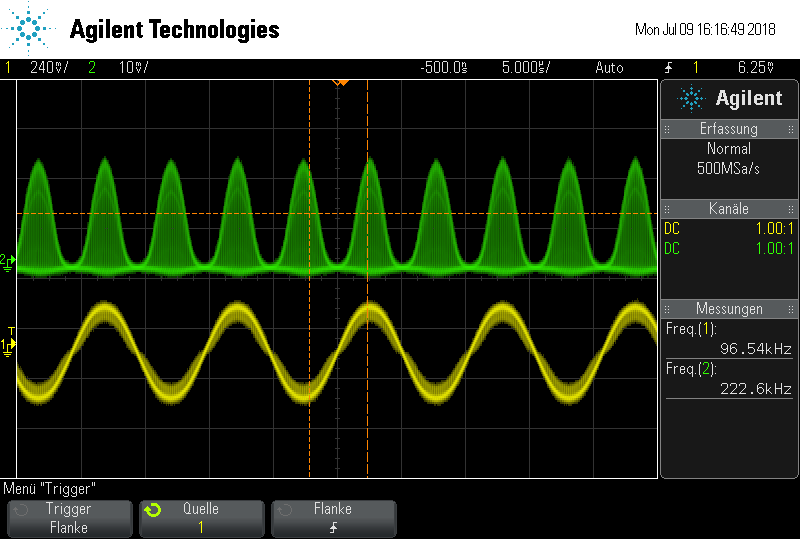
\includegraphics[width=0.7\textwidth]{osci/amp_demod_diode_A.png}
  \caption{Signal $U_{\text{A}}$ am Punkt A bei der Demodulation eines amplitudenmodulierten Signales mit Hilfe einer
  Diode und einem Tiefpass nach Schaltung \ref{fig:8}.}
  \label{fig:diode_punkt_A}
\end{figure}


\begin{figure}
  \centering
  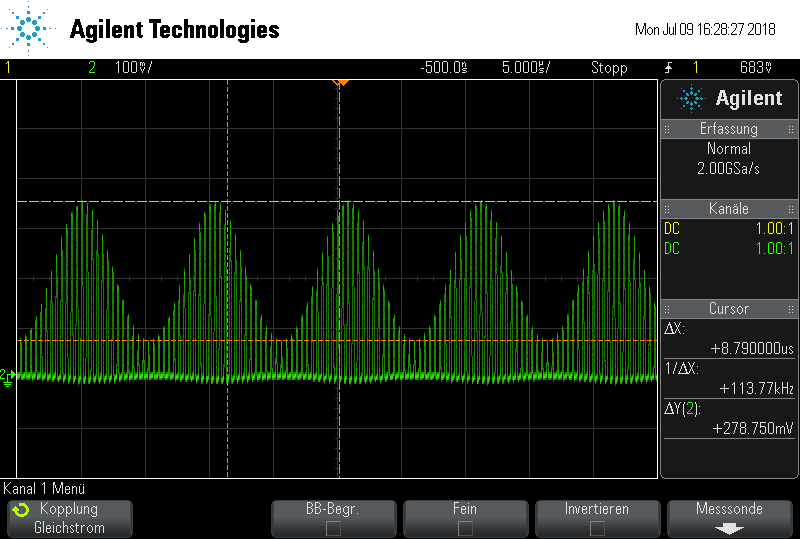
\includegraphics[width=0.7\textwidth]{osci/amp_demod_diode.png}
  \caption{Demoduliertes Signal eines amplitudenmodulierten Signales mit Hilfe einer
  Diode und einem Tiefpass nach Schaltung \ref{fig:8}.}
\label{fig:diode_demod_amp}
\end{figure}

Zu beobachten ist, dass das demodulierte Signal eine doppelt so große Frequenz
und eine zwei Großenordung kleinere Amplitude als das Ausgangssignal
besitzt.

\FloatBarrier
\subsection{(h) Demodulation einer frequenzmodulierten Schwingung
mit Hilfe eines Flankendemodulators}
\label{subsec:auswertung_h}
Die Abbildung \ref{fig:freq_zu_amp}
zeigt ein amplitudenmoduliertes Signal, das aus einem LC-Schwingkreis
wie in Schaltung \ref{fig:11} und einem frequenzmodulierten Signal wie in Abbildung
\ref{fig:freq_zeit} zu sehen, erzeugt wurde.
Aufgrund des verwendeten LC-Schwingkreises, der eine Resonanzfrequenz $f_{res}< \SI{1}{\mega\hertz}$ besitzt,
wird die abfallende Flanke der Resonanzkurve zur Umwandelung von
frequenzmodulierten zu amplitudenmodulierten Signal genutzt,
da die Trägerfrequenz
aufgrund des Laufzeitkabel nur $f_{\text{T}}=\SI{1.00(5)}{\mega\hertz}$ betragen darf.
Dies hat zu folge, dass eine Phase von $\SI{180}{\degree}$ zwischen demoduliertem und Ausgangssignal
erwartet wird.
Als Modulationsfrequenz dient wieder $f_{\text{M}}=\SI{0.10(1)}{\mega\hertz}$.

Das so erzeugt amplitudenmodulierte Signal wird wie in Kapitel \ref{subsubsec:auswertung_g}
mit einer Diode und einem Tiefpass demoduliert, zu sehen in Abbildung \ref{fig:demod_frequenz}.
Jedoch ist die erwartete Phasenverschiebung nicht deutlich erkennbar.


\begin{figure}
  \centering
  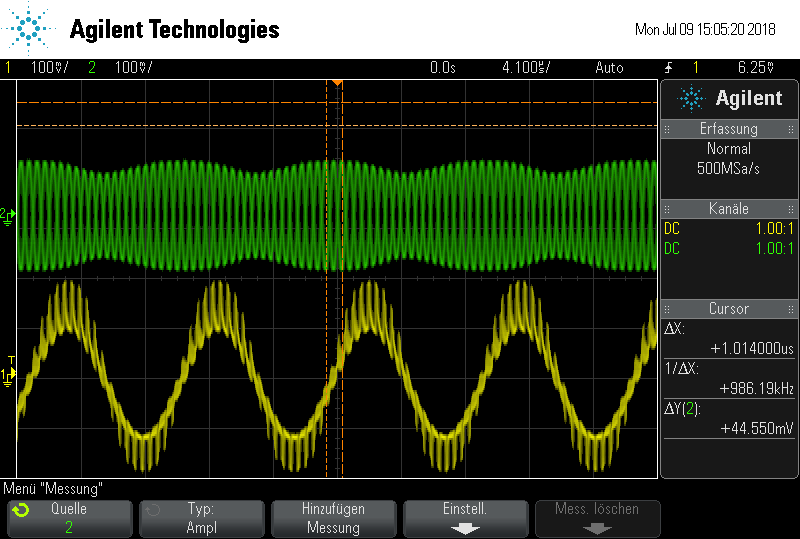
\includegraphics[width=0.7\textwidth]{osci/freq_demod_amp.png}
  \caption{Umwandelung eines Frequenzmodulierten Signales in ein Amplitudenmoduliertes
Signal mit durch einen LC-Schwingkreis nach Abbildung \ref{fig:11}.}
\label{fig:freq_zu_amp}
\end{figure}



\begin{figure}
  \centering
  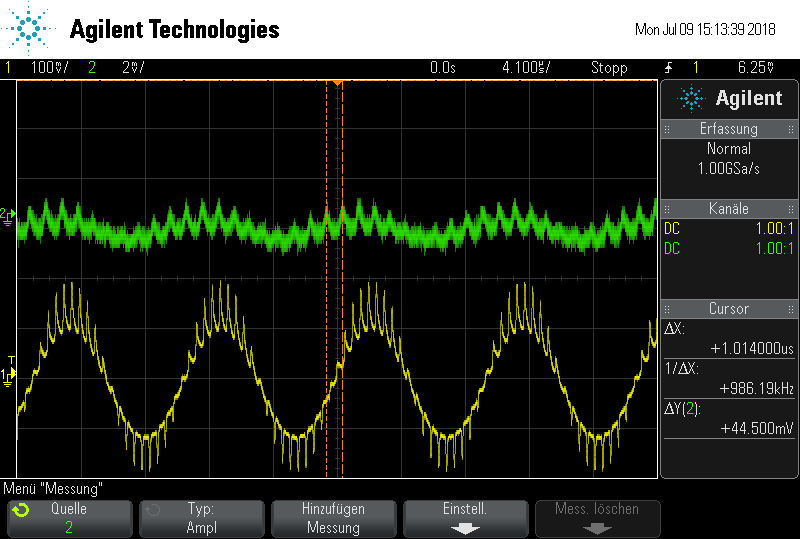
\includegraphics[width=0.7\textwidth]{osci/freq_demod.png}
  \caption{Demodulierung eines frequenzmodulierten Signales
  mit der Schaltung \ref{fig:flankenmodulator}.}
\label{fig:demod_frequenz}
\end{figure}
